\actTitle{1.6 - Transfomations of Graphs}

\videoLink{Section 1.6 Day 1}{https://www.youtube.com/playlist?list=PLYHZK3b8UFw3srUWdN3pnV1WRNsEcqx-T}
% \videoLink{Section 1.6 Day 2}{https://www.youtube.com/playlist?list=PLYHZK3b8UFw3PC3qUoQPSdpFhzCqjRG8m}

\noindent \textbf{Topics:}  basic functions, vertical translations and scaling, horizontal translations and scaling, horizontal and vertical reflections, graphing transformations\\

\noindent \textbf{Student Learning Outcomes:}
\begin{enumerate}
\item (In class) Students will be able to recognize basic functions.
\item Students will be able to transform graphs of functions.
\item Students will be able to graph a function based on transformations.
\end{enumerate}

\hrule 

\bigskip


\subsection{Vertical and Horizontal Shifts} ~

\hspace{-.4in} \begin{tabular}{| l |} \hline \underline{Vertical shifts.} Assume that $c$ is a positive number. \\
The graph of $y = f(x)+c$ is obtained from the graph of $y=f(x)$ by shifting it $c$ units upward. \\
The graph of $y = f(x)-c$ is obtained from the graph of $y=f(x)$ by shifting it $c$ units downward.
 \\ \hline
\end{tabular}

\begin{enumerate}

\item For this problem, let $f(x)=x^2$. Sketch the graph of the function $y=f(x) - 3$. Compare the domains and ranges of $y=f(x)$ and $y=f(x)-3$.



      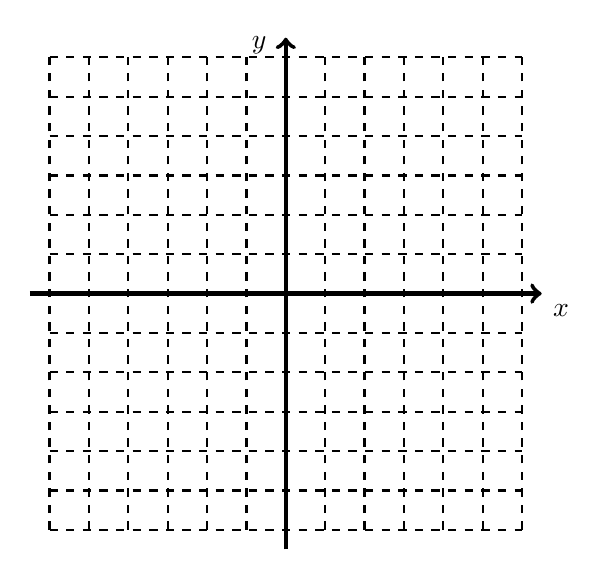
\begin{tikzpicture}[y=0.5cm, x=0.5cm,font=\sffamily]
        \begin{scope} %[shift={(0,8)}]
          %% ticks
          \draw[xstep = 1, ystep=1.0,black,dashed,thick] % very thin,opacity=0.85,
                 (-6.0,-6.0) grid ( 6.0, 6.0);
             %% axis
           \draw[ultra thick,->] (-6.5,0) -- coordinate (x axis mid) (6.5,0)
                node[anchor = north west] {$x$}; 
           \draw[ultra thick,->] (0,-6.5) -- coordinate (y axis mid) (0,6.5) 
                node[anchor = east,shift={(-0.2,-0.2)}]  {$y$};

           %\foreach \y in {-1,1,...,4} {
           %   \draw (1pt, \y) -- (-1pt, \y) node[yshift=-6,xshift=1,anchor=west] {$\y$};
           % }
           %\foreach \x in {-3,-2,-1,1,2,3} {
           %   \draw (\x,1pt) -- (\x,-1pt) node[yshift=-5,xshift=-1,anchor=east] {$\x$};
           % }

          \end{scope}
        \end{tikzpicture}



\newpage
\hspace{-.4in} \begin{tabular}{| l |} \hline \underline{Horizontal shifts.} Assume that $c$ is a positive number. \\
The graph of $y = f(x-c)$ is obtained from the graph of $y=f(x)$ by shifting it $c$ units to the right. \\
The graph of $y = f(x+c)$ is obtained from the graph of $y=f(x)$ by shifting it $c$ units to the left.
 \\ \hline
\end{tabular} 

\item Convince yourself that the rule above is correct by using the example $f(x)=x^2.$ Sketch the graph of $y = f(x -2)$ on the axes below.

      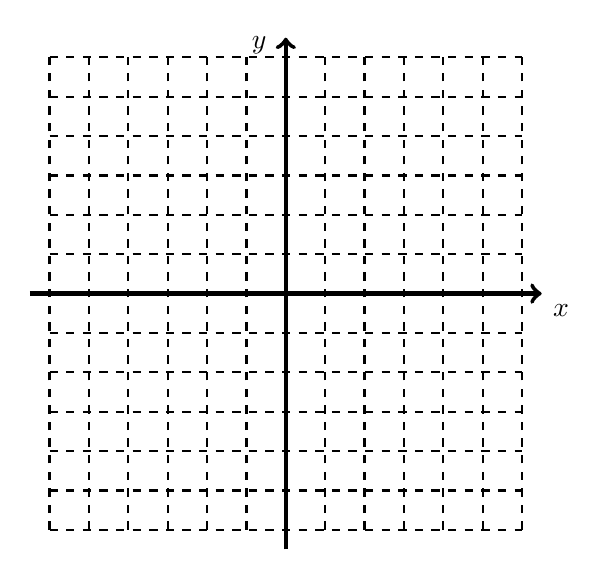
\begin{tikzpicture}[y=0.5cm, x=0.5cm,font=\sffamily]
        \begin{scope} %[shift={(0,8)}]
          %% ticks
          \draw[xstep = 1, ystep=1.0,black,dashed,thick] % very thin,opacity=0.85,
                 (-6.0,-6.0) grid ( 6.0, 6.0);
             %% axis
           \draw[ultra thick,->] (-6.5,0) -- coordinate (x axis mid) (6.5,0)
                node[anchor = north west] {$x$}; 
           \draw[ultra thick,->] (0,-6.5) -- coordinate (y axis mid) (0,6.5) 
                node[anchor = east,shift={(-0.2,-0.2)}]  {$y$};

           %\foreach \y in {-1,1,...,4} {
           %   \draw (1pt, \y) -- (-1pt, \y) node[yshift=-6,xshift=1,anchor=west] {$\y$};
           % }
           %\foreach \x in {-3,-2,-1,1,2,3} {
           %   \draw (\x,1pt) -- (\x,-1pt) node[yshift=-5,xshift=-1,anchor=east] {$\x$};
           % }

          \end{scope}
        \end{tikzpicture}


\item Compare the domains and ranges of $y = \sqrt{x}$ and $f(x)=\sqrt{x+4}$. Think about why this makes sense and is consistent with the shifting.\\[2in]



\item If the point $(3, -4)$ is on the graph of $y = f(x)$, find the corresponding point on the graph of $y = f(x - 5)+3$. \\

\newpage

\subsection{Reflection, Compression, and Stretching} ~

\hspace{-.4in} \begin{tabular}{| l |} \hline \underline{Reflection through the $x$-axis.} The graph of $y=-f(x)$ is obtained by reflecting the graph of $y=f(x)$ \\ through the $x$-axis.
 \\ \hline
\end{tabular} 


\vspace{-.1in}
\item For the graph of $y=f(x)$ shown below, sketch the graph of $y=-f(x)$.

  \noindent
      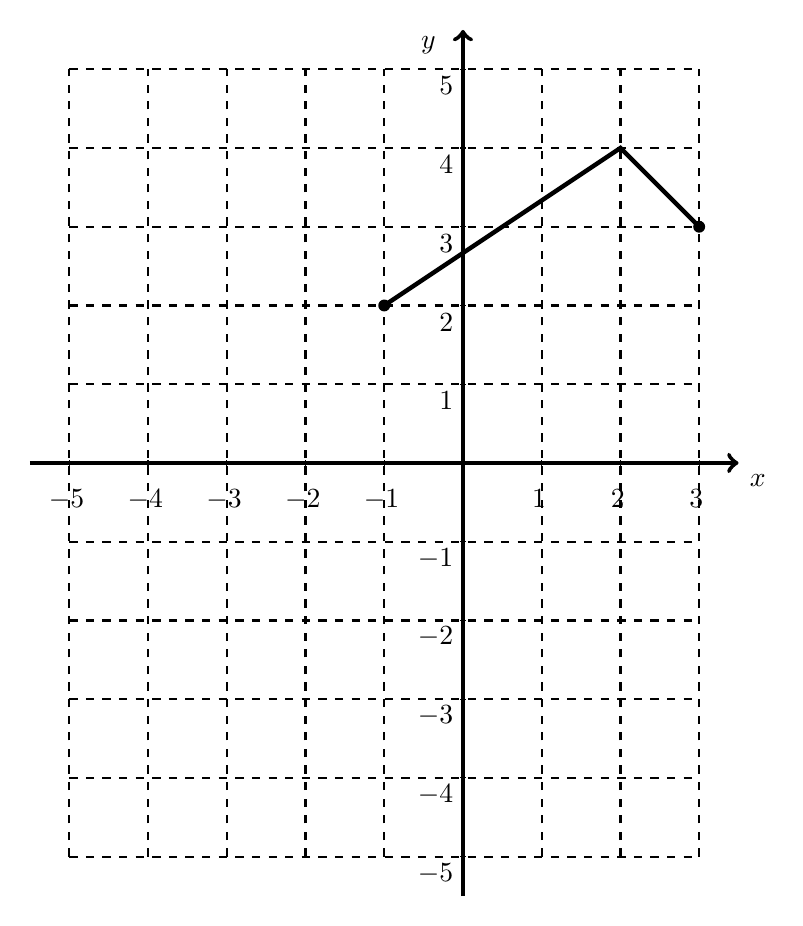
\begin{tikzpicture}[y=1cm, x=1cm,font=\sffamily]
        \begin{scope} %[shift={(0,8)}]
          %% ticks
          \draw[xstep = 1, ystep=1.0,black,dashed,thick] % very thin,opacity=0.85,
                 (-5.0,-5.0) grid ( 3.0, 5.0);
             %% axis
           \draw[ultra thick,->] (-5.5,0) -- coordinate (x axis mid) (3.5,0)
                node[anchor = north west] {$x$}; 
           \draw[ultra thick,->] (0,-5.5) -- coordinate (y axis mid) (0,5.5) 
                node[anchor = east,shift={(-0.2,-0.2)}]  {$y$};

           \foreach \y in {-5,...,-1,1,2,3,4,5} {
              \draw (1pt, \y) -- (-1pt, \y) node[yshift=-6,xshift=1,anchor=east] {$\y$};
            }
           \foreach \x in {-5,-4,...,-1,1,2,3} {
              \draw (\x,1pt) -- (\x,-1pt) node[yshift=-5,xshift=-1,anchor=north] {$\x$};
            }

            \draw[ultra thick] (-1,2) -- (2,4) -- (3,3);
            \fill[black] (-1,2) circle [radius=0.5ex];
            \fill[black] ( 3,3) circle [radius=0.5ex];
          \end{scope}

        \end{tikzpicture}



\begin{tabular}{| p{0.8\textwidth} |} \hline
\underline{Vertical Compression/Stretching} Assume that $c$ is a
positive number.  If $c>1$, the graph of $y=cf(x)$ is obtained by
stretching the graph of $y=f(x)$ vertically by a factor of $c$.  If
$c$ is between $0$ and $1$, the graph of $y=cf(x)$ is obtained by
compressing the graph vertically by a factor of $1/c$.
 \\ \hline
\end{tabular} 


\vspace{-.1in}
\item If the point $P(3,-1)$ is on the graph of $y=f(x)$, find the corresponding point on the graph of (a) $y = 7f(x)$ and (b) $y = \dfrac{1}{4}f(x)$. \\[.4in]



\newpage
\item For the graph of $y=f(x)$ shown below, sketch the graph of $y=2f(x+3)-1$. \\
%\noindent Hint: work in stages, one modification at a time. Use order of operations to make your stages.\\
\scalebox{0.25}{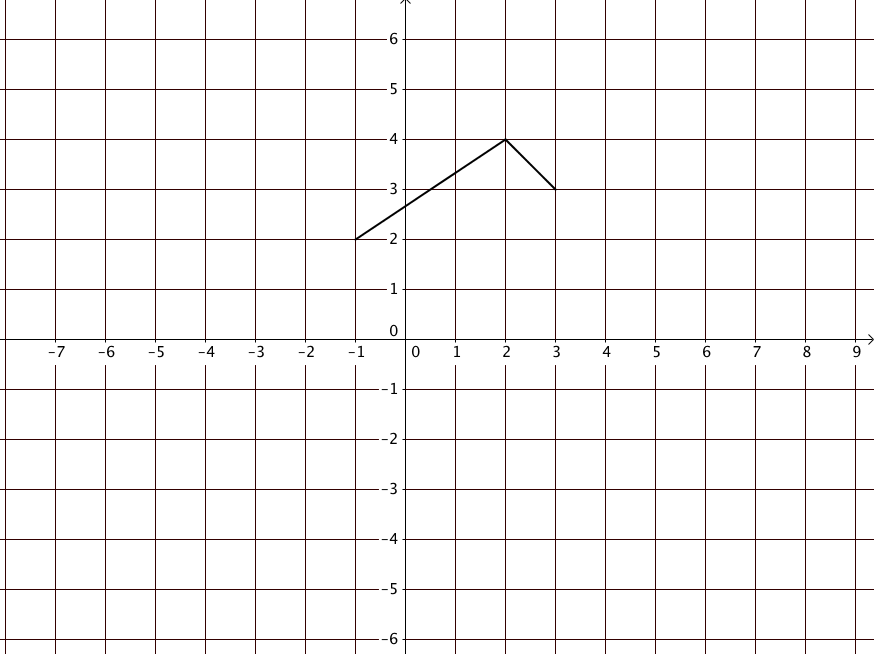
\includegraphics{pwshift}} 
%\end{enumerate}
%
%
%
%
%\noindent MATH 1113 - Alli  \hfill Section 2.5 - Graphs of Functions\\
%\noindent Part 2 \\
%\noindent Topics: reflections of graphs, stretching/compressing of graphs   \\



\begin{tabular}{| l |} \hline \underline{Reflection through the $y$-axis.} The graph of $y=f(-x)$ is obtained by reflecting the graph of $y=f(x)$ \\ through the $y$-axis.
 \\ \hline
\end{tabular} 

%\begin{enumerate}
\vspace{-.1in}
\item For the graph of $y=f(x)$ shown below, sketch the graph of $y=f(-x)$.\\
\scalebox{0.5}{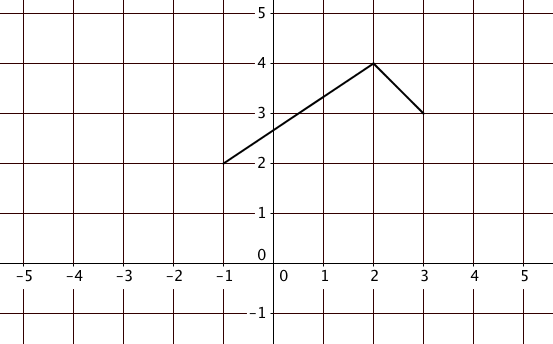
\includegraphics{pwshift4}} 






\hspace{-.4in} \begin{tabular}{| l |} \hline \underline{Horizontal Compression/Stretching} Assume that $c$ is a positive number. \\
If $c>1$, the graph of $y=f(cx)$ is obtained by compressing the graph horizontally by a factor $c$. \\
If $c$ is between $0$ and $1$, the graph of $y=f(cx)$ is obtained by stretching the graph of $y=f(x)$ \\ horizontally by a factor of $1/c$.
 \\ \hline
\end{tabular} 

\vspace{-.1in}
\item For the graph of $y=f(x)$ shown below, sketch the graph of $y=f(2x)$.\\
\scalebox{0.3}{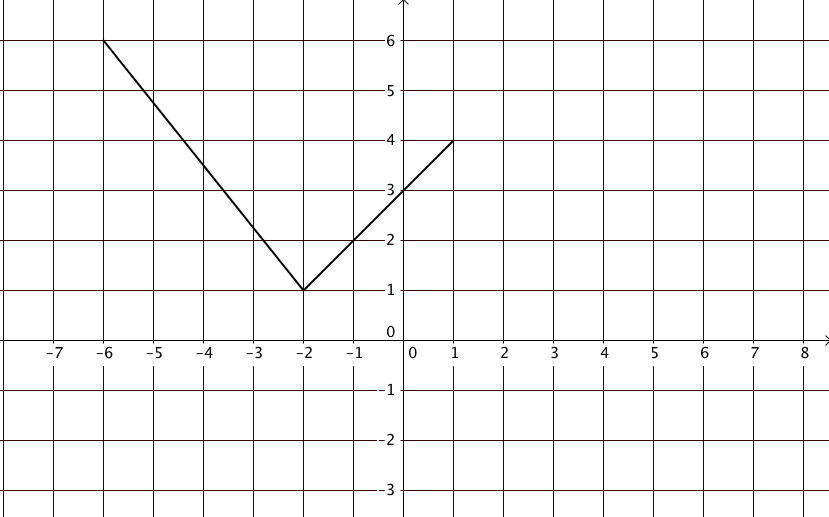
\includegraphics{pwshift2}} 

\newpage
\item For the graph of $y=f(x)$ shown below, sketch the graph of $y = |f(x)|$.\\
\scalebox{0.3}{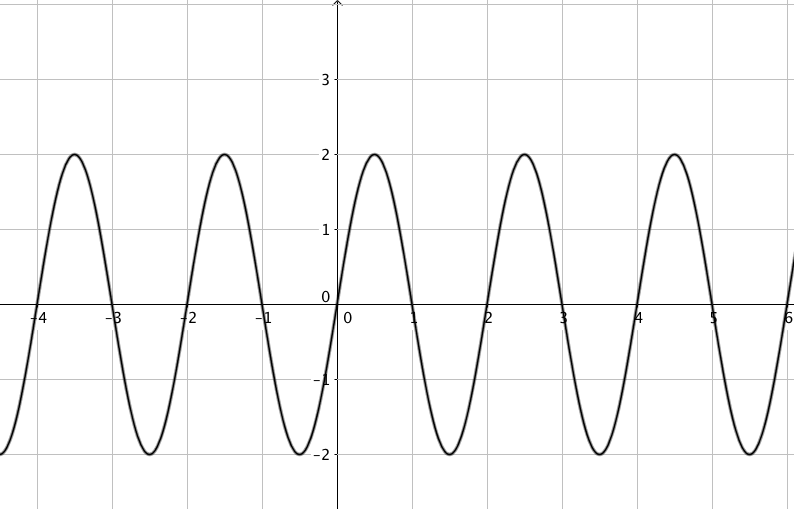
\includegraphics{sineflip}} \\[2in]





\end{enumerate}

\noindent \textbf{Student Learning Outcomes Check}

\begin{enumerate}
\item Can you transform graphs of functions?
\item Do you understand the difference between a shift and a reflection?  Or vertical and horizontal transformations?
\end{enumerate}

\noindent \textbf{If any of your answers were no, please ask about these topics in class.}



